\section{T\"atigkeiten w\"ahrend des Praktikums}
\subsection{Organisation und Bewerbung}
%------------------------------------------------------------------------
\mode<presentation>{
  \begin{frame}[t] \frametitle{Organisation und Bewerbung}
    \vspace{0.5cm}
    \begin{itemize}
      \item Praktikumsbeschreibung: Implementierung von kartenbezogenen Algorithmen (in C++)
      \item Zeitraum von ungef\"ahr 5 Monaten
      \item Vollzeit: 39 h/Woche mit bestimmten Kernzeiten
      \item verg\"utet
      \item regelm\"a\ss ige Abstimmung mit Betreuer
        \vspace{0.5cm}
      \item Bewerbungsprozess:
        \begin{itemize}
        \item Bewerbung um ausgeschriebene Praktikumsstelle (\url{https://recruiting.fraunhofer.de/}) %Bewerbung im Zeitraum Mitte-März
        \item Bewerbungsgespr\"ach mit sp\"ateren Betreuer
        \end{itemize}
    \end{itemize}
  \end{frame}
}

\subsection{Aufgabenbeschreibung}
%------------------------------------------------------------------------
\begin{frame}[t] \frametitle{Aufgabenbeschreibung}
  \begin{itemize}
  \item Implementierung von kartebezogenen Algorithmen f\"ur ein Softwareframework im Bereich der C2X-Kommunikation
    \begin{itemize}
    \item {\usebeamercolor[fg]{structure}Routing-Algorithmen:} Bestimmung des ``besten'' Weges zwischen zwei Positionen
    \item {\usebeamercolor[fg]{structure}Mapmatching-Algorithmen:} Abgleich von Kartenmaterial und Standortdaten (GPS-Position)
    \end{itemize}
  \item Implementierung und Test von ausgew\"ahlten Algorithmen
  \end{itemize}
  \begin{columns}
    \begin{column}{0.35\textwidth}
      \begin{itemize}
      \item M\"ogliche Anwendungsf\"alle: 
        \begin{itemize}
        \item \emph{mobincity} (EU-Projekt)
        \item \emph{Adaptive City mobility} (nationales Projekt)
        \item ...
        \end{itemize}
      \end{itemize}
    \end{column}
    \begin{column}{0.6\textwidth}
      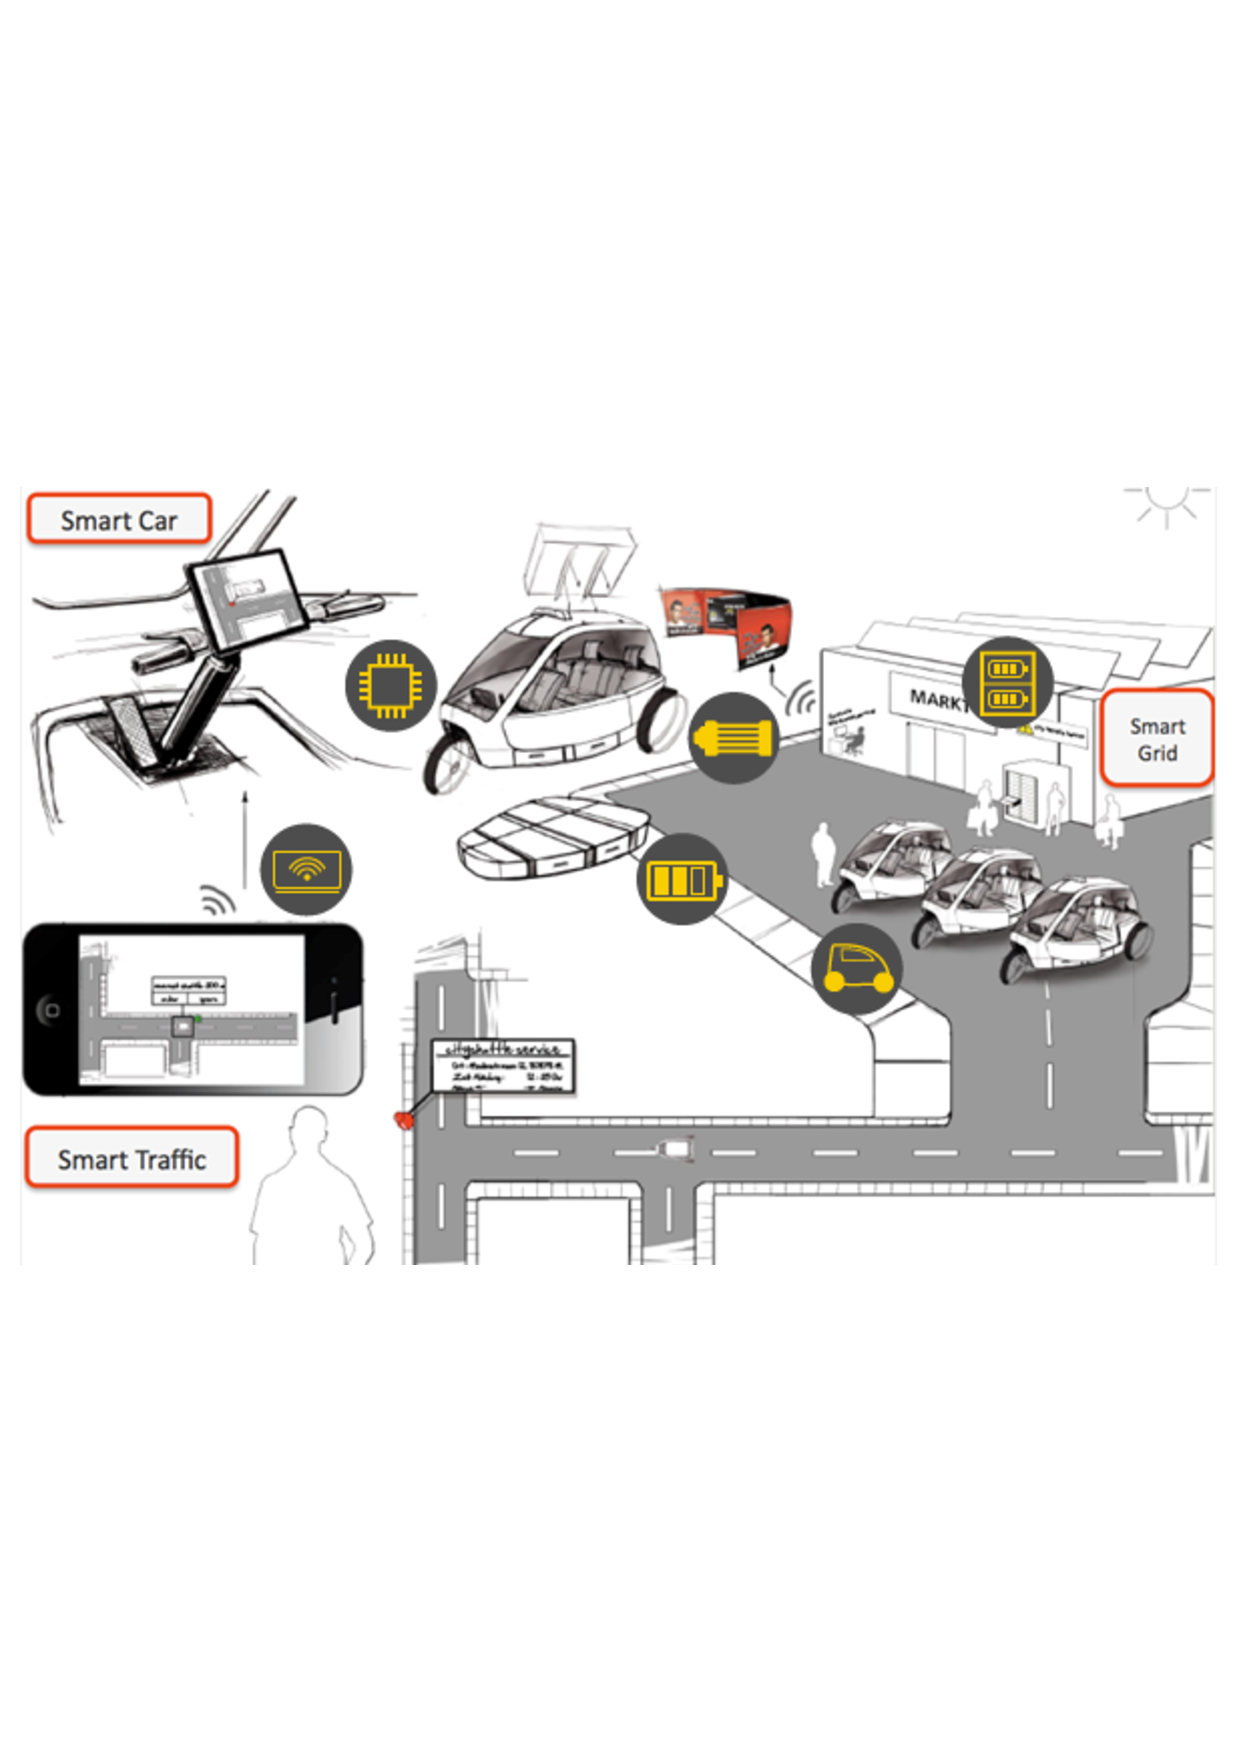
\includegraphics[width=1\textwidth]{pics/acmFraunhofer}
    \end{column}
  \end{columns}
\end{frame}

%------------------------------------------------------------------------
\begin{frame}[t] \frametitle{Arbeitsprozess}
\vspace{0.5cm}
  \begin{itemize}
  \item bereits vorhandenes Framework:
    \begin{itemize}
    \item linzenzkostenfreies Kartenmaterial vom OpenStreetMap-Projekt (osm-Files)
    \item Framework zum Einlesen des Kartenmaterials
    \end{itemize}
  \item Arbeitsprozess:
    \begin{itemize}
    \item Selbstst\"andige Recherche (Internet, Paper)
    \item Entwurf eines Software-Modells
    \item Anpassung und Implementierung
    \item Tests
    \end{itemize}
  \item kleinere Nebent\"atigkeiten
  \end{itemize}
\end{frame}

\subsection{Routing}
%------------------------------------------------------------------------
\begin{frame} \frametitle{Implementierung von Routing-Algorithmen}
  \begin{itemize}
    \item Grundlage: angepasster Dijkstra-Algorithmus
      \begin{itemize}
      \item Abbiegeverbote (Routing \"uber Kanten anstatt Knoten)
      \item Einbahnstra\ss en
      \item Kreisverkehre
      \end{itemize}
      \vspace{0.1cm}
    \item Verbesserung der Laufzeit durch bidirektionale Suche
      \vspace{0.1cm}
    \item Verbesserung des Dijkstra-Algorithmus durch Heuristiken (Sch\"atzfunktionen): Verbesserung der Laufzeit
      \begin{itemize}
      \item euklidische Heuristik: A*-Algorithmus
      \item Landmarken-Heuristik (ben\"otigt Vorberechnung): ALT-Algorithmus
      \end{itemize}
      \vspace{0.1cm}
    \item Kombination von bidirektionaler Suche und Heuristiken
  \end{itemize}
\end{frame}

\begin{frame}[t] \frametitle{Routing-Beispiel}
  \begin{columns}
    \begin{column}{0.3\textwidth}
      \includegraphics<1-3>[width=1\textwidth]{pics/dijkstraFraunhofer}      
    \end{column}
    \begin{column}{0.3\textwidth}
      \includegraphics<2-3>[width=1\textwidth]{pics/biDijkstraFraunhofer}      
    \end{column}
    \begin{column}{0.3\textwidth}
      \includegraphics<3>[width=1\textwidth]{pics/altFraunhofer}      
    \end{column}
  \end{columns}
\end{frame}

\subsection{Mapmatching}
% ------------------------------------------------------------------------
\begin{frame} \frametitle{Implementierung von Mapmatching-Algorithmen}
  \begin{itemize}
  \item einfache geometrische Mapmatching-Algorithmen:
    \begin{itemize}
    \item Matching auf n\"achstgelegenen Knoten
    \item Matching auf n\"achstgelegene Kante (``orthogonale'' Projektion)
    \end{itemize}
  \item topologischer Mapmatching-Algorithmus: berechnet wahrscheinlichste Match-Position durch zus\"atzliche Kriterien:
    \begin{itemize}
    \item Zusammenhang von Stra\ss enabschnitten, Abbiegeverbote
    \item Kurs-Informationen
    \item Geschwindigkeitsdaten
    \end{itemize}
  \item MHT Mapmatching (multiple-hypothesis-technique)
    \begin{itemize}
    \item \"ahnlich zum topologischen Mapmatcher
    \item betrachtet mehrere Kandidaten-Routen gleichzeitig
    \end{itemize}
  \end{itemize}
\end{frame}

\begin{frame}[t] \frametitle{Mapmatching-Beispiele}
  \begin{columns}
    \begin{column}{0.45\textwidth}
      \includegraphics<1-2>[width=1\textwidth]{pics/pointRoadFraunhofer}
    \end{column}
    \begin{column}{0.45\textwidth}
      \includegraphics<2>[width=1\textwidth]{pics/weightTopoFraunhofer}
    \end{column}
  \end{columns}
\end{frame}